\setbackground
{
	\centering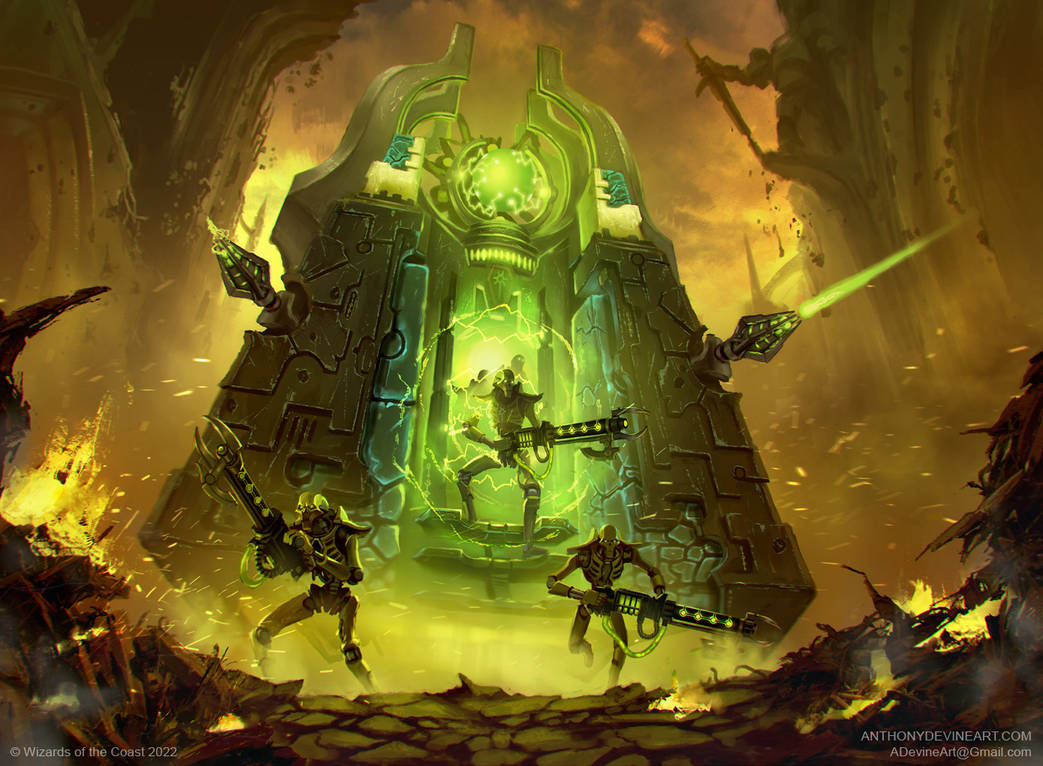
\includegraphics[height=400pt, width=400pt]{heavy_art.jpg}
	\subsection{\texorpdfstring{\centering\Huge Heavy Support}{Heavy Support}}
	
	\centerline{\begin{minipage}{400pt}
			\centering
			"We thought in terms of wars. Of destruction. Of conquest. But eternity also requires what you would call...entertainment."
			
			\vspace*{1em}
			\raggedleft Djoseras
	\end{minipage}}
}

\newpage
\clearbackground
\subsubsection[Canoptek Doomstalker Patrol]{}

\fbox{\begin{imgminipage}{marble.jpg}[t]{0.2\textwidth}
		\color{white}
		\centering {\large HEAVY SUPPORT}
		
		\color{black}
\end{imgminipage}}
\hspace{0.5em}
\begin{minipage}[t]{0.72\textwidth}
	{\large \textbf{Canoptek Doomstalker Patrol \dotfill X Points}}
	
	\begin{tabular}{m{165 pt} *{10}{c}}
		& M & WS & BS & S & T & W & I & A & Ld & Sv \\
		\hline
		Canoptek Doomstalker & 10 & 3 & 3 & 6 & 6 & 6 & 2 & 3 & 10 & 3+ \\
	\end{tabular}
	\small
	\begin{minipage}[t]{0.5\textwidth}
		\begin{flushleft}
			\vspace*{2em}
			\textbf{Unit Composition}
			\begin{itemize}
				\item 1 Canoptek Doomstalker
			\end{itemize}
			
			\textbf{Wargear}
			\begin{itemize}
				\item Close Combat Weapon
				\item \quickref{Doomsday Blaster}
				\item Two \quickref{Gauss Flayer}s
			\end{itemize}
		\end{flushleft}
	\end{minipage}
	\begin{minipage}[t]{0.5\textwidth}
		\begin{flushleft}
			\vspace*{2em}
			\textbf{Unit Type}
			\begin{itemize}
				\item Dreadnought (Canoptek, \quickref{Living Metal})
			\end{itemize}
			
			\textbf{Special Rules}
			\begin{itemize}
				\item Containment Field
				\item \quickref{Reanimation Protocols}
				\item Sentinel Protocols
				\item \quickref{Soulles Hordes} (Silver)
			\end{itemize}
		\end{flushleft}
	\end{minipage}
	
	\vspace*{2em}
	\textbf{Weapons}
	
	\begin{tabular}{m{95 pt} *{4}{c} >{\raggedright\arraybackslash}p{130pt}}
		& Range & Type & S & AP & Abilities \\
		\quickref{Doomsday Blaster} & & & & & \\
		— Low Power & 24" & Heavy 1 & 8 & 3 & Blast \\
		— High Power & 48" & Heavy 1 & 10 & 1 & Large Blast, Divert Power \\
		\quickref{Gauss Flayer} & 24" & Rapid Fire & 4 & 5 & \quickref{Gauss} (6+) \\
	\end{tabular}
	
	\vspace*{2em}
	\textbf{Unit Rules}
	
	\textit{Containment Field:} Canoptek Doomstalker models have a 4+ Invulnerable Save and any model with an containment field and a Wounds Characteristic that suffers an unsaved Wound with the Instant Death special rule is not immediately removed as a casualty, but instead loses D3 Wounds instead of one for each unsaved Wound with the Instant Death special rule inflicted on it. In addition, when a model with an containment field loses its last Wound or Hull Point, but before it is removed as a casualty or replaced with a Wreck, all models both friendly and enemy within D6" suffer an automatic Hit at Str 8, AP —. 
	
	\textit{Sentinel Protocols:} %TODO: This
	
	\vspace*{2em}
	\textbf{Options}
	\begin{itemize}
		\item The Canoptek Doomstalker Patrol may include:
		\begin{itemize}
			\item Up to an additional 1 Canoptek Doomstalker \dotfill X points each
		\end{itemize}
	\end{itemize}
\end{minipage}



\newpage
\subsubsection[Doomsday Ark]{}
\fbox{\begin{imgminipage}{marble.jpg}[t]{0.2\textwidth}
		\color{white}
		\centering {\large HEAVY SUPPORT}
		
		\raggedright \small
		\color{black}
\end{imgminipage}}
\hspace{0.5em}
\begin{minipage}[t]{0.72\textwidth}
	{\large \textbf{Doomsday Ark \dotfill X Points}}
	\begin{NiceTabular}{m{145 pt} *{2}{c} | *{3}{c} | c | c }
		& & & \cellgray{3}{Armour} & & & & \cellgray{1}{Transport} \\
		& M & BS & \cellgray{1}{Front} & \cellgray{1}{Side} & \cellgray{1}{Rear} & HP & \cellgray{1}{Capacity} \\
		\hline
		Doomsday Ark & 12 & 4 & \cellgray{1}{11} & \cellgray{1}{11} & \cellgray{1}{11} & 4 &\cellgray{1}{—} \\
	\end{NiceTabular}
	\small
	\begin{minipage}[t]{0.5\textwidth}
		\begin{flushleft}
			\vspace*{2em}
			\textbf{Unit Composition}
			\begin{itemize}
				\item 1 Doomsday Ark
			\end{itemize}
			
			\textbf{Wargear}
			\begin{itemize}
				\item Hull (Front) Mounted \quickref{Doomsday Cannon}
				\item Five Sponson (Left) Mounted \quickref{Gauss Flayer}s
				\item Five Sponson (Right) Mounted \quickref{Gauss Flayer}s
				\item \quickref{Quantum Shielding}
			\end{itemize}
		\end{flushleft}
	\end{minipage}
	\begin{minipage}[t]{0.5\textwidth}
		\begin{flushleft}
			\vspace*{2em}
			\textbf{Unit Type}
			\begin{itemize}
				\item Vehicle (\quickref{Living Metal}, Open-Topped Skimmer)
			\end{itemize}
			
			\textbf{Special Rules}
			\begin{itemize}
				\item \quickref{Awakening Protocols} (Silver)
				\item Power of the Machine Spirit
			\end{itemize}
		\end{flushleft}
	\end{minipage}
	
	\vspace*{2em}
	\textbf{Weapons}
	
	\begin{tabular}{m{95 pt} *{4}{c} >{\raggedright\arraybackslash}p{130pt}}
		& Range & Type & S & AP & Abilities \\
		\hline
		\quickref{Doomsday Cannon} & & & & & \\
		— Low Power & 36" & Heavy 1 & 8 & 3 & Blast \\
		— High Power & 72" & Heavy 1 & 10 & 1 & Large Blast, Divert Power \\
		\quickref{Gauss Flayer} & 24" & Rapid Fire & 4 & 5 & \quickref{Gauss} (6+) \\
	\end{tabular}


	\vspace*{2em}
	\textbf{Options}
	\begin{itemize}
	\item A Doomsday Ark may take:
	\begin{itemize}
		\item \quickref{Quantum Shielding Matrix} \dotfill X points
	\end{itemize} 
	\end{itemize} 
\end{minipage}


\newpage
\subsubsection[Doom Scythe]{}
\fbox{\begin{imgminipage}{marble.jpg}[t]{0.2\textwidth}
		\color{white}
		\centering {\large HEAVY SUPPORT}
		
		\raggedright \small
		\color{black}
\end{imgminipage}}
\hspace{0.5em}
\begin{minipage}[t]{0.72\textwidth}
	{\large \textbf{Doom Scythe \dotfill X Points}}
	\begin{NiceTabular}{m{145 pt} *{2}{c} | *{3}{c} | c | c }
		& & & \cellgray{3}{Armour} & & & & \cellgray{1}{Transport} \\
		& M & BS & \cellgray{1}{Front} & \cellgray{1}{Side} & \cellgray{1}{Rear} & HP & \cellgray{1}{Capacity} \\
		\hline
		Doom Scythe & 24 & 4 & \cellgray{1}{11} & \cellgray{1}{11} & \cellgray{1}{11} & 4 &\cellgray{1}{—} \\
	\end{NiceTabular}
	\small
	\begin{minipage}[t]{0.5\textwidth}
		\begin{flushleft}
			\vspace*{2em}
			\textbf{Unit Composition}
			\begin{itemize}
				\item 1 Doom Scythe
			\end{itemize}
			
			\textbf{Wargear}
			\begin{itemize}
				\item Hull (Front) Mounted \quickref{Heavy Death Ray}
				\item Hull (Front) Mounted Twink-Linked \quickref{Tesla Destructor}
			\end{itemize}
		\end{flushleft}
	\end{minipage}
	\begin{minipage}[t]{0.5\textwidth}
		\begin{flushleft}
			\vspace*{2em}
			\textbf{Unit Type}
			\begin{itemize}
				\item Vehicle (Hover, Flyer, \quickref{Living Metal})
			\end{itemize}
			
			\textbf{Special Rules}
			\begin{itemize}
				\item \quickref{Awakening Protocols} (Silver)
			\end{itemize}
		\end{flushleft}
	\end{minipage}
	
	
	\vspace*{2em}
	\textbf{Weapons}
	
	\begin{tabular}{m{95 pt} *{4}{c} >{\raggedright\arraybackslash}p{130pt}}
		& Range & Type & S & AP & Abilities \\
		\hline
		\quickref{Heavy Death Ray} & 24" & Heavy 1 & 10 & 1 & Blast, Lance \\
		\quickref{Tesla Destructor} & 24" & Heavy 4 & 7 & — & \quickref{Tesla} (6+), Twin-Linked \\
	\end{tabular}
\end{minipage}



\newpage
\subsubsection[Monolith]{}
\fbox{\begin{imgminipage}{marble.jpg}[t]{0.2\textwidth}
		\color{white}
		\centering {\large HEAVY SUPPORT}
		
		\raggedright \small
		\color{black}
\end{imgminipage}}
\hspace{0.5em}
\begin{minipage}[t]{0.72\textwidth}
	{\large \textbf{Monolith \dotfill X Points}}
	\begin{NiceTabular}{m{145 pt} *{2}{c} | *{3}{c} | c | c }
		& & & \cellgray{3}{Armour} & & & & \cellgray{1}{Transport} \\
		& M & BS & \cellgray{1}{Front} & \cellgray{1}{Side} & \cellgray{1}{Rear} & HP & \cellgray{1}{Capacity} \\
		\hline
		Monolith & 12 & 4 & \cellgray{1}{14} & \cellgray{1}{14} & \cellgray{1}{14} & 4 &\cellgray{1}{—} \\
	\end{NiceTabular}
	\small
	\begin{minipage}[t]{0.5\textwidth}
		\begin{flushleft}
			\vspace*{2em}
			\textbf{Unit Composition}
			\begin{itemize}
				\item 1 Monolith
			\end{itemize}
			
			\textbf{Wargear}
			\begin{itemize}
				\item \quickref{Eternity Gate}
				\item Four Hull Mounted \quickref{Gauss Flux Arcs}
				\item Turret Mounted \quickref{Particle Whip}
			\end{itemize}
		\end{flushleft}
	\end{minipage}
	\begin{minipage}[t]{0.5\textwidth}
		\begin{flushleft}
			\vspace*{2em}
			\textbf{Unit Type}
			\begin{itemize}
				\item Vehicle (\quickref{Living Metal}, Skimmer)
			\end{itemize}
			
			\textbf{Special Rules}
			\begin{itemize}
				\item \quickref{Awakening Protocols} (Silver)
				\item Deep Strike
				\item Power of the Machine Spirit
			\end{itemize}
		\end{flushleft}
	\end{minipage}

	\vspace*{2em}
	\textbf{Access Points}
	
	The Monolith has one Access Point on the Front of its hull.
		
	\vspace*{2em}
	\textbf{Weapons}
	
	\begin{tabular}{m{95 pt} *{4}{c} >{\raggedright\arraybackslash}p{130pt}}
		& Range & Type & S & AP & Abilities \\
		\hline
		\quickref{Gauss Flux Arcs} & 24" & Heavy 3 & 4 & 5 & \quickref{Gauss} (6+) \\
		\quickref{Particle Whip} & 24" & Ordnance 1 & 8 & 3 & Discriminatory, Large Blast \\
	\end{tabular}
\end{minipage}



\newpage
\subsubsection[Tesseract Ark]{}
